\noindent
{}
\begin{allparts}
\part
Explain how the hadron wavefunction
$$\psi_\mathrm{hadron} = \psi_\mathrm{space}\psi_\mathrm{spin}\psi_\mathrm{flavour}\psi_\mathrm{colour}$$
leads to the prediction of an octet of spin-$\frac 1 2$ states and a decuplet of spin-$\frac 3 2$ states for the
lowest-mass baryons formed from up, down and strange quarks.\marks{6}
\ANS{BOOKWORK: Standard from the lecture notes.}
\part
Briefly explain the origin of the baryon mass formula
$$M_{qqq} = m_1 +m_2 +m_3 +A'\left[
\frac{\vec S_1 \cdot \vec S_2}{m_1 m_2}
+
\frac{\vec S_2 \cdot \vec S_3}{m_2 m_3}
+
\frac{\vec S_3 \cdot \vec S_1}{m_3 m_1}
\right],$$
where $A'$ is a constant.\marks{2}
\ANS{BOOKWORK: Standard from the lecture notes.}
\part
Derive the specific form  the above mass formula takes for the  case of a spin-$\frac 1 2$ baryon composed of one up and two strange quarks. Repeat this exercise to determine how the mass of a spin-$\frac 3 2$  bound state with the same quark content depends on the same quantities.  \shorthint{In both cases show your working and leave each answer in terms of $m_u$, $m_s$ and $A'$ only.}  \marks{8}

\ANS{

The answer is:

\begin{align*}
M_{uss} & =
\begin{cases}m_u + 2m_s + A'\left[
\frac 1 {4 m_s^2} - \frac 1 {m_u m_s} \right]
& \text{for $J^P={\frac1 2}^+$ and}
\\
 m_u + 2m_s + A'\left[
\frac 1 {4 m_s^2} + \frac 1 {2m_u m_s}\right] & \text{for $J^P={\frac3 2}^+$.}
\end{cases}
\end{align*}

The derivation follows.


There are two like-flavour quarks ($ss$) and one other-flavour quark ($u$). Label the three quarks `1', `2' and `$u$' with the numbers distinguishing the two $s$-quarks.

The `hard' part of this calculation is finding 
$$
\frac{\vec S_1 \cdot \vec S_2}{m_1 m_2}
+
\frac{\vec S_2 \cdot \vec S_3}{m_2 m_3}
+
\frac{\vec S_3 \cdot \vec S_1}{m_3 m_1}.
$$
Fortunately we do not need to compute each of  $\vec S_1\cdot \vec S_2$, $\vec S_1\cdot \vec S_3$ and $\vec S_2\cdot \vec S_3$ separately.  Because:
\begin{align}
\frac{\vec S_1 \cdot \vec S_2}{m_1 m_2}
+
\frac{\vec S_2 \cdot \vec S_3}{m_2 m_3}
+
\frac{\vec S_3 \cdot \vec S_1}{m_3 m_1}
&=
\frac{\vec S_1 \cdot \vec S_2}{m_s^2}
+
\frac{\vec S_2 \cdot \vec S_u}{m_s m_u}
+
\frac{\vec S_u \cdot \vec S_1}{m_u m_s}\nonumber
\\
&=
\frac{\vec S_1 \cdot \vec S_2}{m_s^2}
+
\frac{\left(\vec S_1+\vec S_2\right) \cdot \vec S_u}{m_u m_s}\label{eq:forsubback}
\end{align}
we only need to compute $\vec S_1 \cdot \vec S_2$ and $\left(\vec S_1+\vec S_2\right) \cdot \vec S_u$.


We recall from the earlier discussion of hadron wavefunctions that we need to consider wave functions for which the FLAVOUR*SPIN parts are symmetric overall. It is not possible to have wave functions which are flavour-odd with respect to the two like-flavour $s$-quarks, and so the resulting flavour-even wavefunction needs to be combined with one which is has an even (i.e. triplet) spin wave function (such as  $\phi^{\text{spin}}_{1 2}=\frac 1 {\sqrt 2} ( \uparrow \downarrow + \downarrow \uparrow)$ or  $\uparrow\uparrow$ or $\downarrow\downarrow$) for quarks `1' and `2'.  I.e. $S_{12}=1$. The difference between the $J=\frac 1 2$ and $J=\frac 3 2$ states will thus be created by  the third quark (the $u$) adding its own $S_3=S_u=\frac 1 2$ either destructively or constructively to the mix.

Considering just the two like quarks we have:
\begin{align}
\vec S_{12}^2 
&= 
\vec S_1^2 +
\vec S_2^2 +
2\vec S_1\cdot \vec S_2
\end{align}
which gives:
\begin{align}
\vec S_1\cdot \vec S_2
&=
\frac 1 2 \left(
\vec S_{12}^2 
-
\vec S_1^2 -
\vec S_2^2 \nonumber
\right)\\
&=
\frac 1 2
\left(
S_{12}(S_{12}+1)
-
S_{1}(S_{1}+1)
-
S_{2}(S_{2}+1)\nonumber
\right)\\
&=
\frac 1 2
\left(
1
\times(1+1)
-
{\frac 1 2}\times({\frac 1 2}+1)
-
{\frac 1 2}\times({\frac 1 2}+1)
\right)\nonumber
\\
&= \frac 1 4 \label{eq:quarter}
\end{align}
which is one of the two main things we set out to find.

Using the above we can then move on and find $\left( \vec S_1+\vec S_2\right) \cdot \vec S_u$ via
\begin{align*}
\vec S^2 
&= 
\vec S_1^2 +
\vec S_2^2 +
\vec S_u^2 +
2 \left( \vec S_1+\vec S_2\right) \cdot \vec S_u 
+ 2\vec S_1\cdot \vec S_2
\end{align*}
which tells us that
\begin{align*}
\left( \vec S_1+\vec S_2\right) \cdot \vec S_u 
&=
\frac 1 2
\left(
\vec S^2 -\left(\vec S_1^2 +
\vec S_2^2 +
\vec S_u^2\right)
-2 \vec S_1\cdot \vec S_2
\right)
\\
&=
\frac 1 2 \left(
J(J+1) - 3\times\left(\frac 1 2 \times \left(\frac 1 2 + 1\right)\right) -
2\times \frac 1 4
\right)
\\
&=
\frac 1 2 J (J+1) - \frac {11}8
\\
&=\begin{cases}
-1 & \text{when $J=\frac 1 2$}\\
+\frac 1 2 & \text{when $J=\frac 3 2$.}\\
\end{cases}
\end{align*}
We can now substitute the values we have just computed for $\vec S_1 \cdot \vec S_2$ and $\left(\vec S_1+\vec S_2\right) \cdot \vec S_3$ back into equation (\ref{eq:forsubback}) and put it together with the (trivial) mass terms to get the baryon mass formulae  given at the start of this answer.
}
\part
The $\Xi^0$ ($J^P={\frac1 2}^+$) and $\Xi^{*0}$ ($J^P={\frac3 2}^+$) baryons are bound states of $uss$ quarks.  Using your formulae from part (c), calculate numerical values for mass predictions for the $\Xi^0$ and $\Xi^{*0}$. \shorthint{The quark masses may be taken to be $m_u = 362~\mathrm{MeV}$ and $m_s = 537~\mathrm{MeV}$.  $A' = 0.026~\mathrm{GeV}^3$.}\marks{1}

\part
The experimentally measured values of the masses are $M(\Xi^0)=1314.86\pm0.20$~MeV and $M(\Xi^{*0})=1531.79\pm0.34$~MeV.  What level of agreement between predicted and measured masses might one reasonably expect the baryon mass formula to provide, and is the level of agreement you saw in (d) better or worse than this?\marks{2}
%
%\noindent



\ANS{

THIS IS THE ANSWER TO (d) and (e) TOGETHER


To three significant figures\footnote{Aside: these answers are probably right to three sig figs (even though the quantity $A'$ is only given to two significant figures) since $A'$ controls the difference (about 200 MeV) between the two values for $M_{uss}$ -- while the absolute value is in the region of 1000 MeV and is controlled by $m_u$ and $m_s$ which were given to higher precision. The prediction (looking at just the maths and error propagation, but ignoring systematic uncertainties) ought therefore to be good to $\pm10$~MeV.} the baryon mass formula just derived yields:  $M(\Xi^0)\sim 1320$~MeV and $M(\Xi^{*0})\sim 1530$~MeV.  These  values are compatible with the experimental results to within the computed values' stated precisions. If anything, the surprise here is that the computed values are so close.  The model is very simple (totally ignoring gluons, sea quarks, and  myriad other non-perturbative effects).  Not only that, but quark masses themselves are very much measurement-method-dependent (since colour confinement prevents quarks from being isolated), so one does not have much confidence that the supplied quark masses are even meaningful for this problem. Most baryon mass predictions are therefore not this good, and this level of agreement is therefore much better than we have a right to expect.
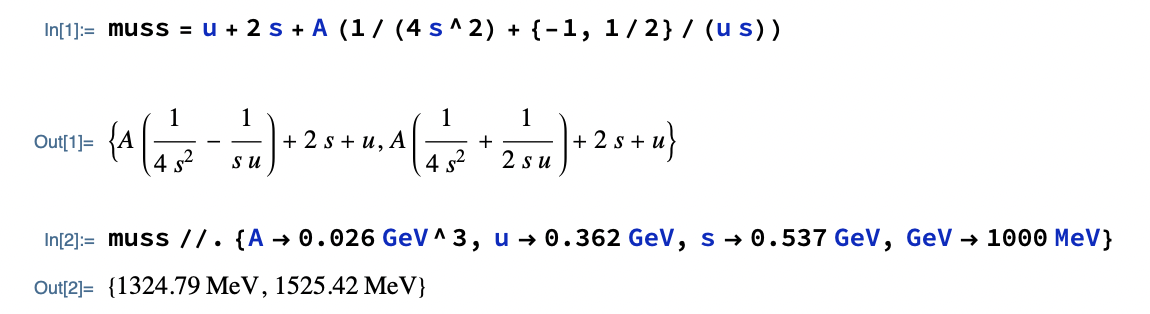
\includegraphics[width=0.7\textwidth]{Images/baryon_mass_calc.png}

}

\end{allparts}


%\begin{allparts}
%\part
%\end{allparts}
